%%%%%%%%%%%%%%%%%%%%%%%%%%%%%%%%%%%%%%%%%
% Beamer Presentation
% LaTeX Template
% Version 1.0 (10/11/12)
%
% This template has been downloaded from:
% http://www.LaTeXTemplates.com
%
% License:
% CC BY-NC-SA 3.0 (http://creativecommons.org/licenses/by-nc-sa/3.0/)
%
%%%%%%%%%%%%%%%%%%%%%%%%%%%%%%%%%%%%%%%%%

%----------------------------------------------------------------------------------------
%	PACKAGES AND THEMES
%----------------------------------------------------------------------------------------

\documentclass[UTF8,aspectratio=169,12pt]{ctexbeamer}

\usepackage{hyperref}
\hypersetup{
	colorlinks=true,
	linkcolor=red,
	anchorcolor=blue,
	citecolor=green
}

\mode<presentation> {
	
	% The Beamer class comes with a number of default slide themes
	% which change the colors and layouts of slides. Below this is a list
	% of all the themes, uncomment each in turn to see what they look like.
	
	%\usetheme{default}
	%\usetheme{AnnArbor}
	%\usetheme{Antibes}
	%\usetheme{Bergen}
	%\usetheme{Berkeley}
	%\usetheme{Berlin}
	%\usetheme{Boadilla}
	%\usetheme{CambridgeUS}
	%\usetheme{Copenhagen}
	%\usetheme{Darmstadt}
	%\usetheme{Dresden}
	%\usetheme{Frankfurt}
	%\usetheme{Goettingen}
	%\usetheme{Hannover}
	%\usetheme{Ilmenau}
	%\usetheme{JuanLesPins}
	%\usetheme{Luebeck}
	\usetheme{Madrid}
	%\usetheme{Malmoe}
	%\usetheme{Marburg}
	%\usetheme{Montpellier}
	%\usetheme{PaloAlto}
	%\usetheme{Pittsburgh}
	%\usetheme{Rochester}
	%\usetheme{Singapore}
	%\usetheme{Szeged}
	%\usetheme{Warsaw}
	
	% As well as themes, the Beamer class has a number of color themes
	% for any slide theme. Uncomment each of these in turn to see how it
	% changes the colors of your current slide theme.
	
	%\usecolortheme{albatross}
	%\usecolortheme{beaver}
	%\usecolortheme{beetle}
	%\usecolortheme{crane}
	%\usecolortheme{dolphin}
	%\usecolortheme{dove}
	%\usecolortheme{fly}
	%\usecolortheme{lily}
	%\usecolortheme{orchid}
	%\usecolortheme{rose}
	%\usecolortheme{seagull}
	%\usecolortheme{seahorse}
	%\usecolortheme{whale}
	%\usecolortheme{wolverine}
	
	%\setbeamertemplate{footline} % To remove the footer line in all slides uncomment this line
	%\setbeamertemplate{footline}[page number] % To replace the footer line in all slides with a simple slide count uncomment this line
	
	%\setbeamertemplate{navigation symbols}{} % To remove the navigation symbols from the bottom of all slides uncomment this line
}

\usepackage{graphicx} % Allows including images
\graphicspath{{./figs/}}
\usepackage{booktabs} % Allows the use of \toprule, \midrule and \bottomrule in tables
\usepackage{longtable}
\usepackage{xcolor}
\usepackage{minted}
\usepackage{listings}
\lstset{numbers=left, %设置行号位置
	numberstyle=\tiny, %设置行号大小
	keywordstyle=\color{blue}, %设置关键字颜色
	commentstyle=\color[cmyk]{1,0,1,0}, %设置注释颜色
	frame=single, %设置边框格式
	escapeinside=``, %逃逸字符(1左面的键),用于显示中文
	%breaklines, %自动折行
	extendedchars=false, %解决代码跨页时,章节标题,页眉等汉字不显示的问题
	xleftmargin=2em,xrightmargin=2em, aboveskip=1em, %设置边距
	tabsize=4, %设置tab空格数
	showspaces=false %不显示空格
}
% Fonts
% \usepackage{libertine}
% \setmonofont{Courier}
%\setCJKsansfont[ItalicFont=Noto Serif CJK SC Black, BoldFont=Noto Sans CJK SC Black]{Noto Sans CJK SC}


%----------------------------------------------------------------------------------------
%	TITLE PAGE
%----------------------------------------------------------------------------------------

\title[第15讲]{第十五讲 :死锁和并发错误检测} % The short title appears at the bottom of every slide, the full title is only on the title page
\subtitle{第5节:并发错误检测}
\author{向勇、陈渝、李国良} % Your name
\institute[清华大学] % Your institution as it will appear on the bottom of every slide, may be shorthand to save space
{
	清华大学计算机系 \\ % Your institution for the title page
	\medskip
	\textit{xyong,yuchen,liguoliang@tsinghua.edu.cn} % Your email address
}
\date{\today} % Date, can be changed to a custom date

\begin{document}

\begin{frame}
\titlepage % Print the title page as the first slide
\end{frame}

%----------------------------------------------
\begin{frame}
\frametitle{提纲} % Table of contents slide, comment this block out to remove it
\tableofcontents % Throughout your presentation, if you choose to use \section{} and \subsection{} commands, these will automatically be printed on this slide as an overview of your presentation

Ref: Shan Lu, \href{https://s4plus.ustc.edu.cn/_upload/article/files/84/48/964812c049829f4538793b862187/430bcb14-7aa7-4689-b340-9c81e735e5eb.pdf}{Detecting and Fixing Concurrency Bugs}, University of Chicago

\end{frame}
%----------------------------------------------
%%	PRESENTATION SLIDES
%----------------------------------------------
\section{第5节:并发错误检测} % Sections can be created in order to organize your presentation into discrete blocks, all sections and subsections are automatically printed in the table of contents as an overview of the talk
%----------------------------------------------
\subsection{Concurrency Bug} % A subsection can be created just before a set of slides with a common theme to further break down your presentation into chunks
%----------------------------------------------
\begin{frame}[fragile]
    \frametitle{Concurrency bug}
%    \framesubtitle{xxxx}

What ordering is guaranteed?

%% figure
    \begin{figure}
    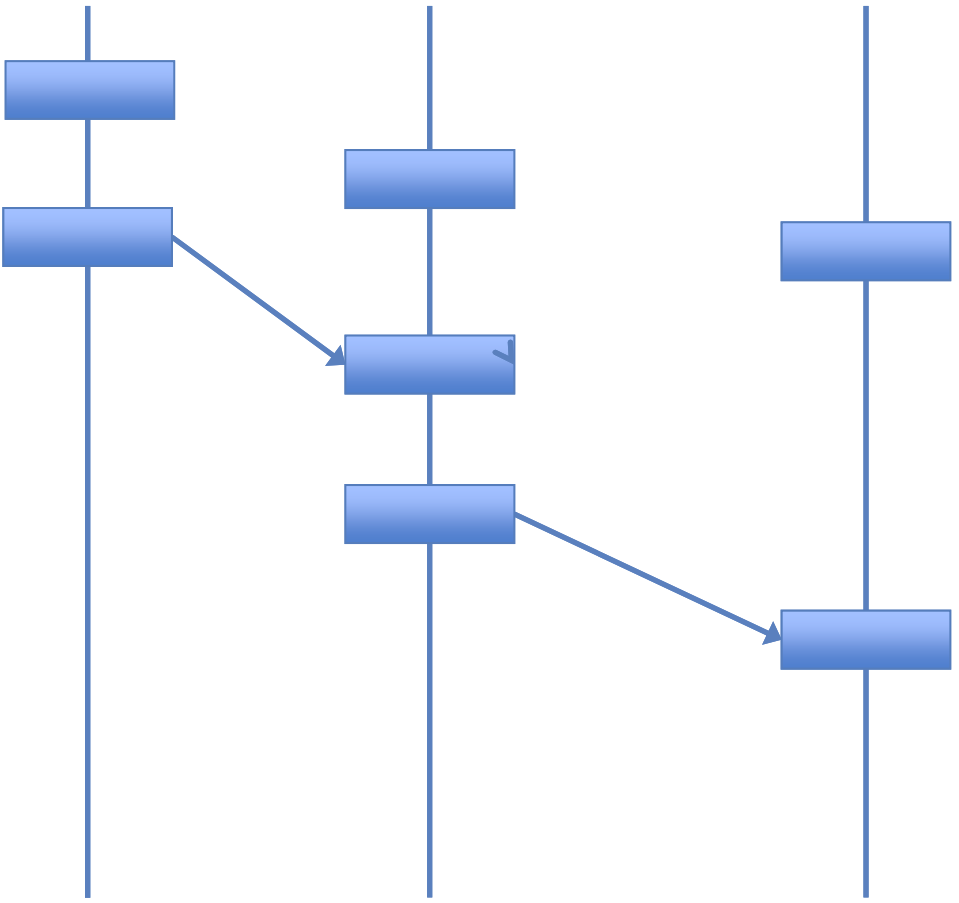
\includegraphics[width=0.45\linewidth]{figs/ordering.png}
%    \caption{xxxx}
    \end{figure}
\end{frame}
%----------------------------------------------
% Shan Lu, Detecting and Fixing Concurrency Bugs, University of Chicago
% 20200407-lecture2.zip-Lec2.pdf
% 
% ### Concurrency bug
% #### Concurrency bug
% 
% 
% 20200407-lecture2.zip-Lec2.pdf-P22
% 
% What ordering is guaranteed?
% 
% ![ordering](figs/ordering.png)
% 
%----------------------------------------------
\begin{frame}[fragile]
    \frametitle{Concurrency bug: Voilation}
%    \framesubtitle{xxxx}
%% figure
    \begin{figure}
    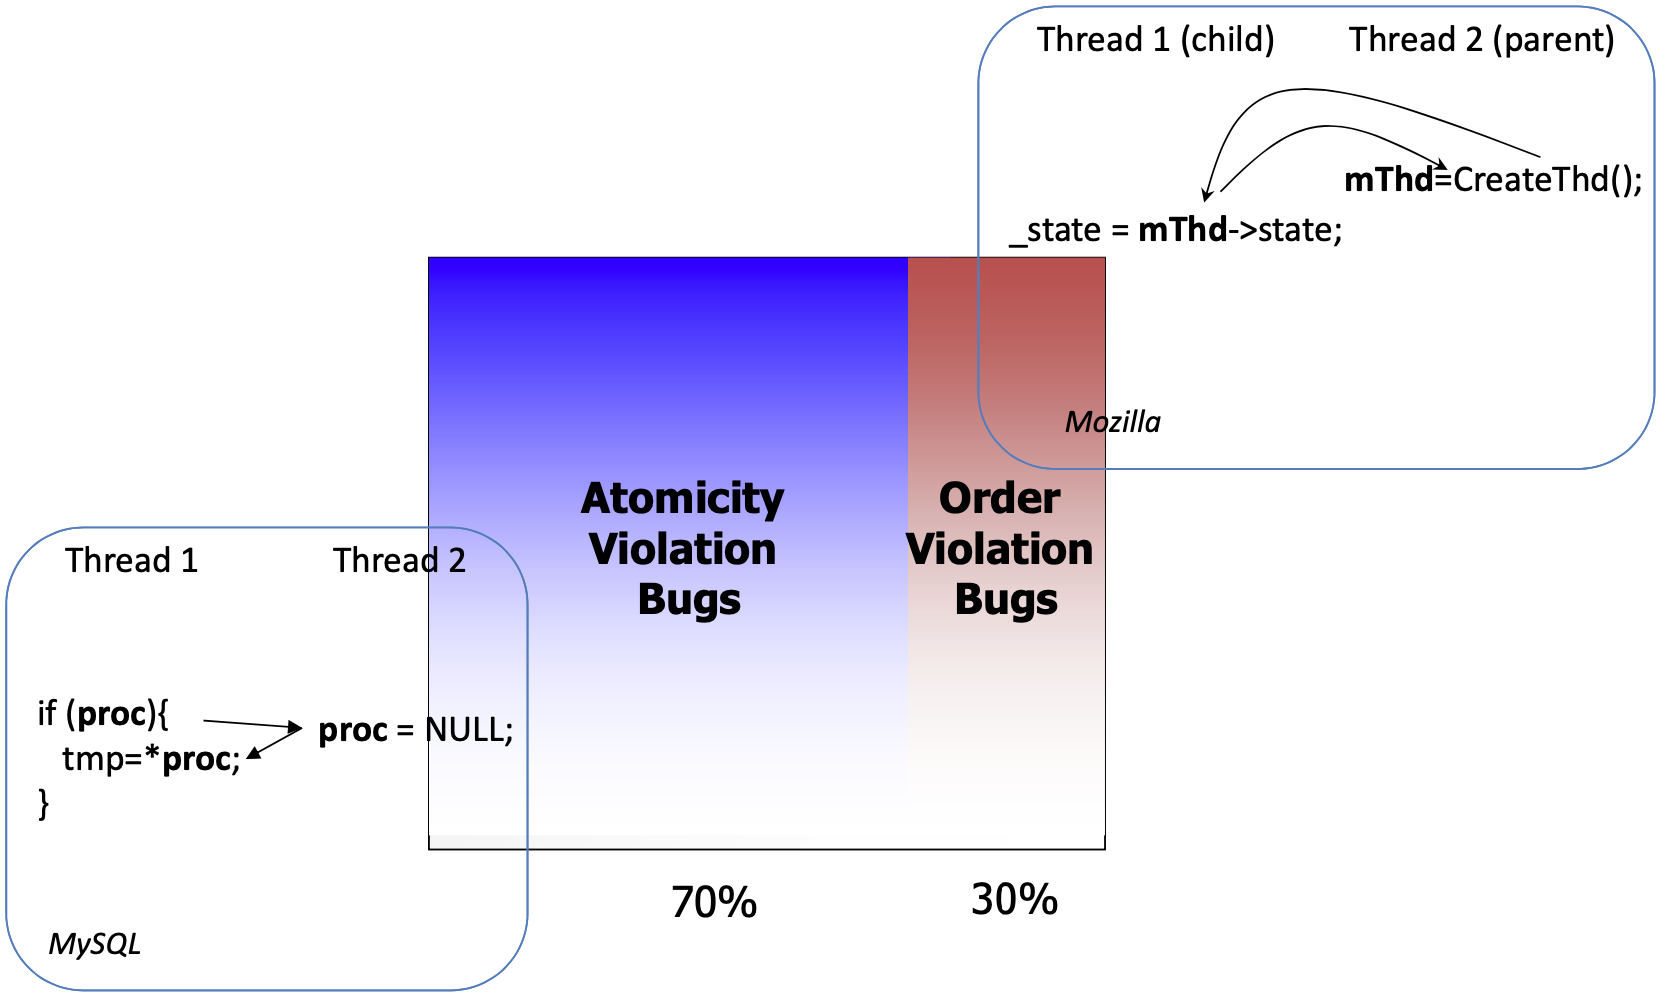
\includegraphics[width=0.75\linewidth]{figs/root-cause-patterns-violation.png}
%    \caption{xxxx}
    \end{figure}
\end{frame}
%----------------------------------------------
% #### Concurrency bug: voilation
% 20200407-lecture2.zip-Lec2.pdf-P40-41
% 
% ![root-cause-patterns-violation](figs/root-cause-patterns-violation.png)
% 
% 
%----------------------------------------------
\begin{frame}[fragile]
    \frametitle{Concurrency bug: Variable}
%    \framesubtitle{xxxx}
%% figure
    \begin{figure}
    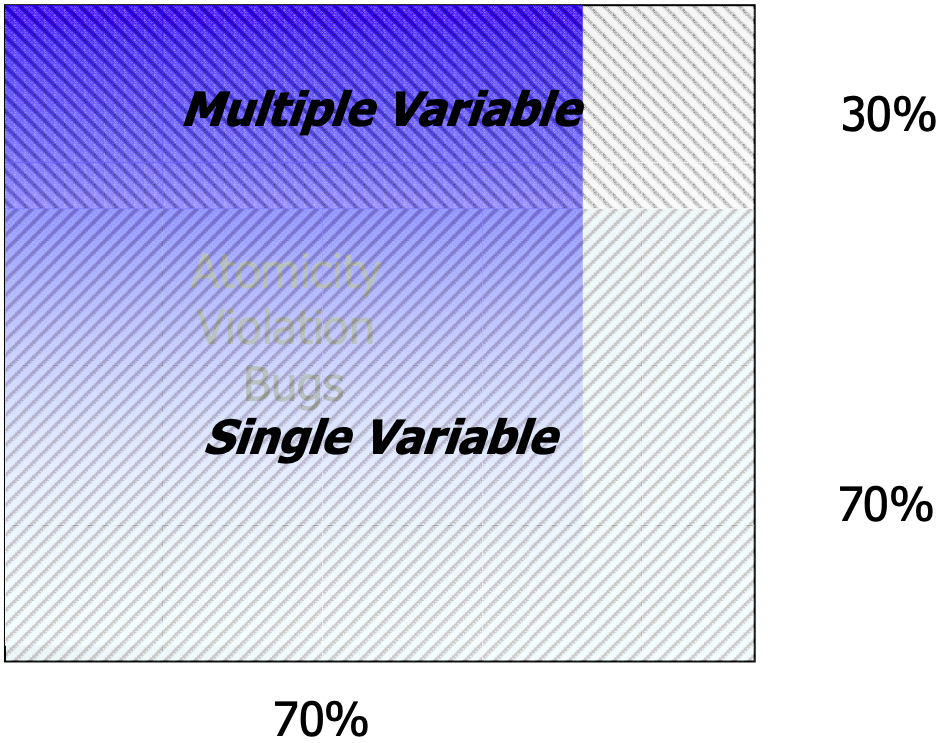
\includegraphics[width=0.56\linewidth]{figs/root-cause-patterns-variable.png}
%    \caption{xxxx}
    \end{figure}
\end{frame}
%----------------------------------------------
% #### Concurrency bug: Variable
% 
% ![root-cause-patterns-variable](figs/root-cause-patterns-variable.png)
% 
%----------------------------------------------
\begin{frame}[fragile]
    \frametitle{Atomicity Violations}
%    \framesubtitle{xxxx}
%% figure
    \begin{figure}
    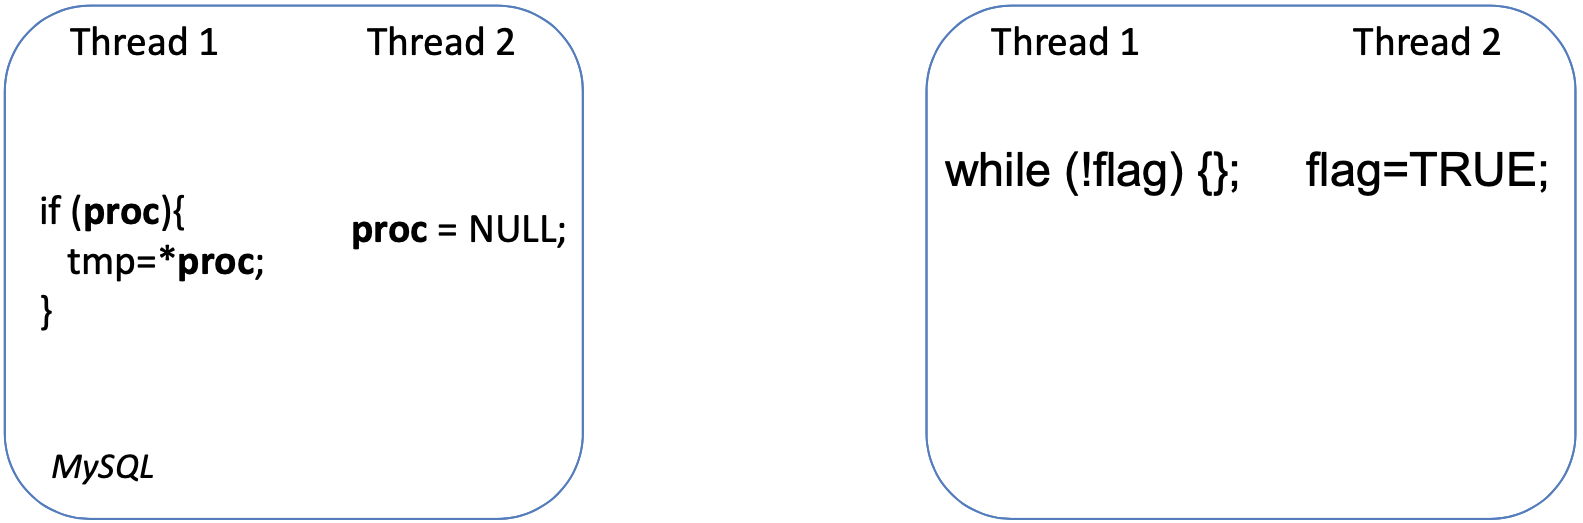
\includegraphics[width=1.0\linewidth]{figs/atomic-region.png}
%    \caption{xxxx}
    \end{figure}
\end{frame}
%----------------------------------------------
% #### Which code regions are expected to be atomic?
% 
% 20200407-lecture2.zip-Lec2.pdf-P47
% 
% ![atomic-region](figs/atomic-region.png)
% 
% 
%----------------------------------------------
\begin{frame}[fragile]
    \frametitle{Order Violations}
%    \framesubtitle{xxxx}
%% figure
    \begin{figure}
    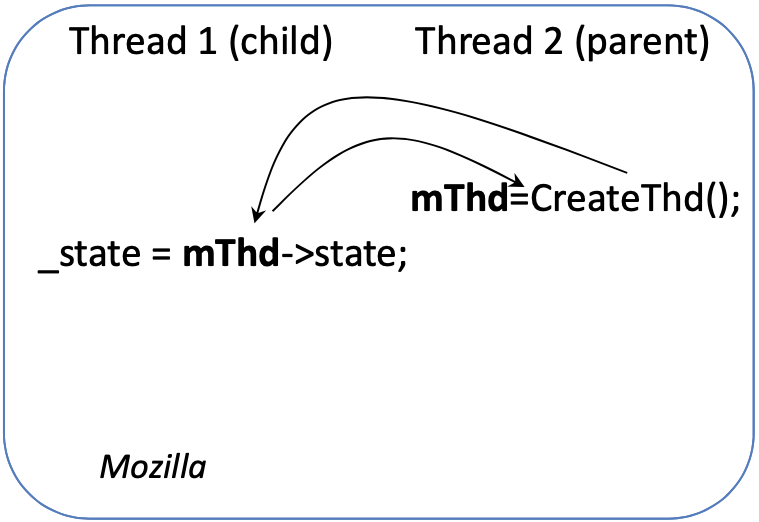
\includegraphics[width=0.65\linewidth]{figs/order-violation.png}
%    \caption{xxxx}
    \end{figure}
\end{frame}
%----------------------------------------------
% #### What are order violations?
% 20200407-lecture2.zip-Lec2.pdf-P51
% 
% ![order-violation](figs/order-violation.png)
% 
%----------------------------------------------
\begin{frame}[fragile]
    \frametitle{Multi‐var Order Violations}
%    \framesubtitle{xxxx}
%% figure
    \begin{figure}
    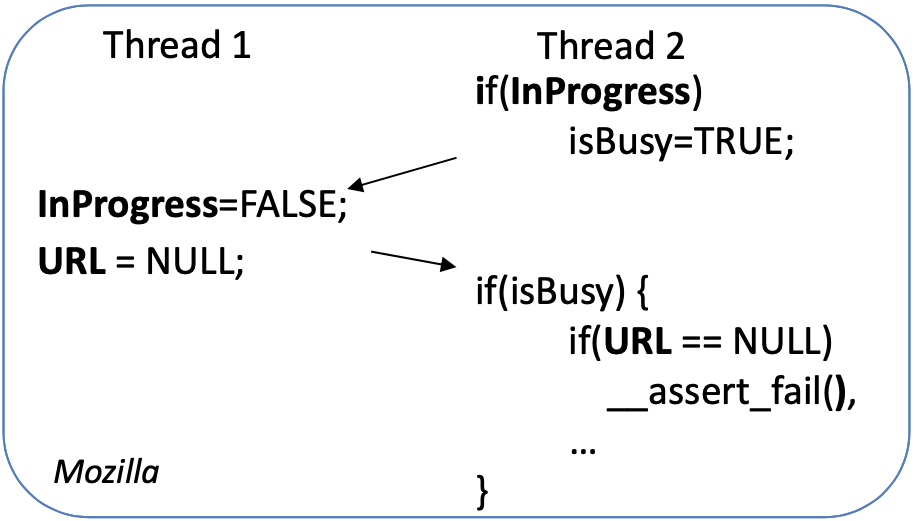
\includegraphics[width=0.8\linewidth]{figs/mutli-variable-ordering-violation.png}
%    \caption{xxxx}
    \end{figure}
\end{frame}
%----------------------------------------------
% #### What are multi‐var order violations?
% 20200407-lecture2.zip-Lec2.pdf-P54
% 
% Untimely accesses to correlated Multiple variables
% 
% ![mutli-variable-ordering-violation](figs/mutli-variable-ordering-violation.png)
% 
% 
%----------------------------------------------
\begin{frame}[fragile]
    \frametitle{The lifecycle of bugs}
%    \framesubtitle{xxxx}
%% figure
    \begin{figure}
    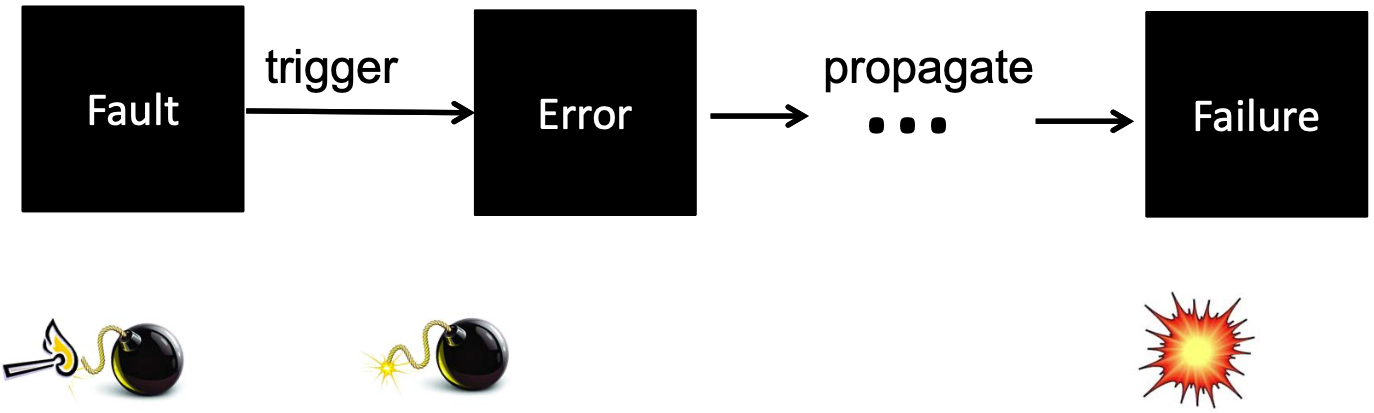
\includegraphics[width=0.9\linewidth]{figs/bug-lifecycle.png}
%    \caption{xxxx}
    \end{figure}
\end{frame}
%----------------------------------------------
% #### The lifecycle of bugs
% 
% 20200407-lecture2.zip-Lec2.pdf-P64
% 
% Data races
% Atomicity violations
% 	single variable
% 	multiple variables
% Order violations
% 
% ![bug-lifecycle](figs/bug-lifecycle.png)
% 
%----------------------------------------------
\begin{frame}
\frametitle{提纲} % Table of contents slide, comment this block out to remove it
\tableofcontents % Throughout your presentation, if you choose to use \section{} and \subsection{} commands, these will automatically be printed on this slide as an overview of your presentation

Ref: Shan Lu, \href{https://s4plus.ustc.edu.cn/_upload/article/files/84/48/964812c049829f4538793b862187/430bcb14-7aa7-4689-b340-9c81e735e5eb.pdf}{Detecting and Fixing Concurrency Bugs}, University of Chicago

\end{frame}
%----------------------------------------------
\subsection{Concurrency Bug Detection} % A subsection can be created just before a set of slides with a common theme to further break down your presentation into chunks
% %----------------------------------------------
% \begin{frame}[fragile]
%     \frametitle{What is the causality relationship here?}
% %    \framesubtitle{xxxx}
%     \begin{columns}
%     \begin{column}{0.5\textwidth}
%         Example1
% 
%     %% figure
%         \begin{figure}
%         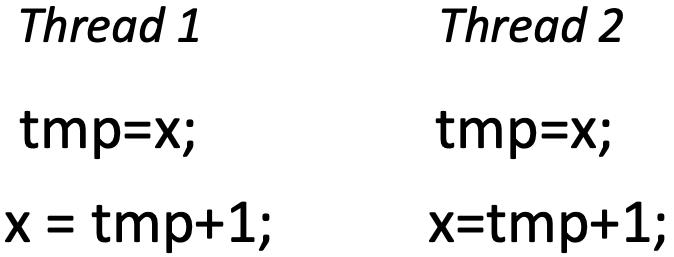
\includegraphics[width=0.7\linewidth]{figs/data-race-example-1.png}
%     %    \caption{xxxx}
%         \end{figure}
%         
% 	\end{column} \pause
%     \begin{column}{0.5\textwidth}
% 
%         Example2
% 
% %% figure
%     \begin{figure}
%     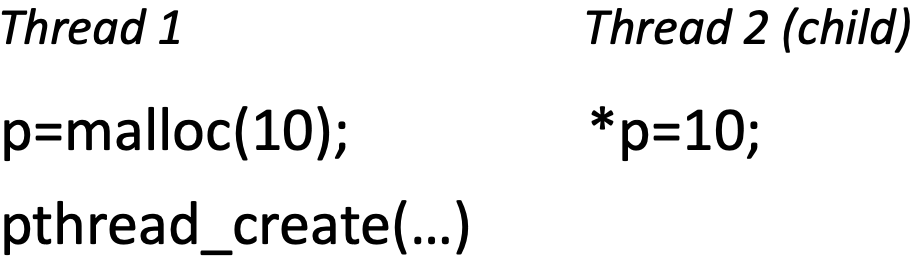
\includegraphics[width=0.85\linewidth]{figs/data-race-example-2.png}
% %    \caption{xxxx}
%     \end{figure}
% 
% \end{column}
% 	\end{columns}
% \end{frame}
% %----------------------------------------------
% ### Concurrency bug detection
% 
% #### What is the causality relationship here?
% 20200407-lecture2.zip-Lec2.pdf-P28
% 
% Example1
% 
% ![data-race-example-1](figs/data-race-example-1.png)
% 
% Example2
% 
% ![data-race-example-2](figs/data-race-example-2.png)
% 
%----------------------------------------------
\begin{frame}[fragile]
    \frametitle{logical clock algorithm}
%    \framesubtitle{xxxx}

Use logic time‐stamps to find concurrent accesses
\pause
%% figure
    \begin{figure}
    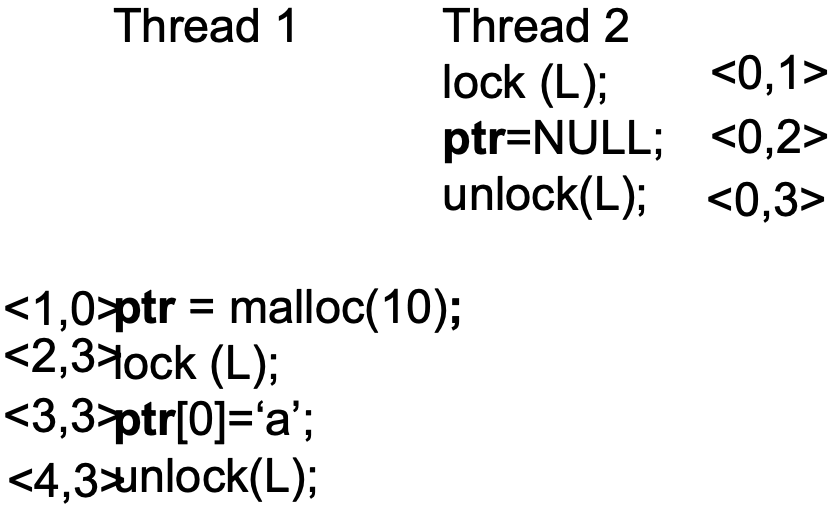
\includegraphics[width=0.45\linewidth]{figs/Happen‐before.png}
%    \caption{xxxx}
    \end{figure}
\end{frame}
%----------------------------------------------
% ####  How to detect data races? Happen‐before algorithm
% 
% 20200407-lecture2.zip-Lec2.pdf-P31
% 
% Use logic time‐stamps to find concurrent accesses
% 
% ![Happen‐before](figs/Happen‐before.png)
% 
%----------------------------------------------
\begin{frame}[fragile]
    \frametitle{Lock‐set algorithm}
%    \framesubtitle{xxxx}

A common lock should protect all conflicting accesses to a shared variable
\pause
%% figure
    \begin{figure}
    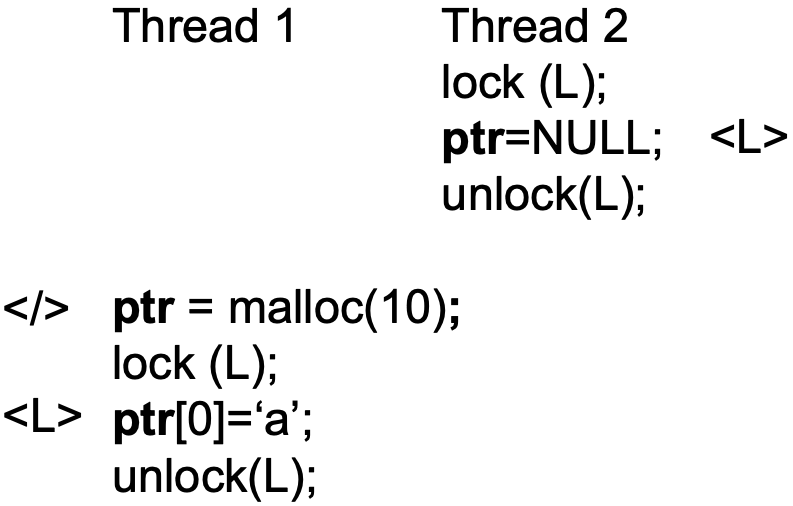
\includegraphics[width=0.5\linewidth]{figs/Lock‐set.png}
%    \caption{xxxx}
    \end{figure}
\end{frame}
%----------------------------------------------
% #### How to detect data races? Lock‐set algorithm
% 20200407-lecture2.zip-Lec2.pdf-P33
% 
% A common lock should protect all conflicting accesses to a shared variable
% 
% ![Lock‐set](figs/Lock‐set.png)
% 
%----------------------------------------------
\begin{frame}[fragile]
    \frametitle{How to detect atomicity‐violations?}
%    \framesubtitle{xxxx}

Know which code region should maintain atomicity

    \begin{figure}
    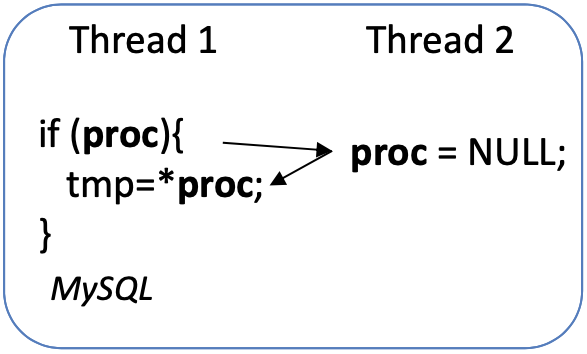
\includegraphics[width=0.27\linewidth]{figs/atomicity.png}
%    \caption{xxxx}
    \end{figure} \pause

Judge whether a code region’s atomicity is violated

%% figure
    \begin{figure}
    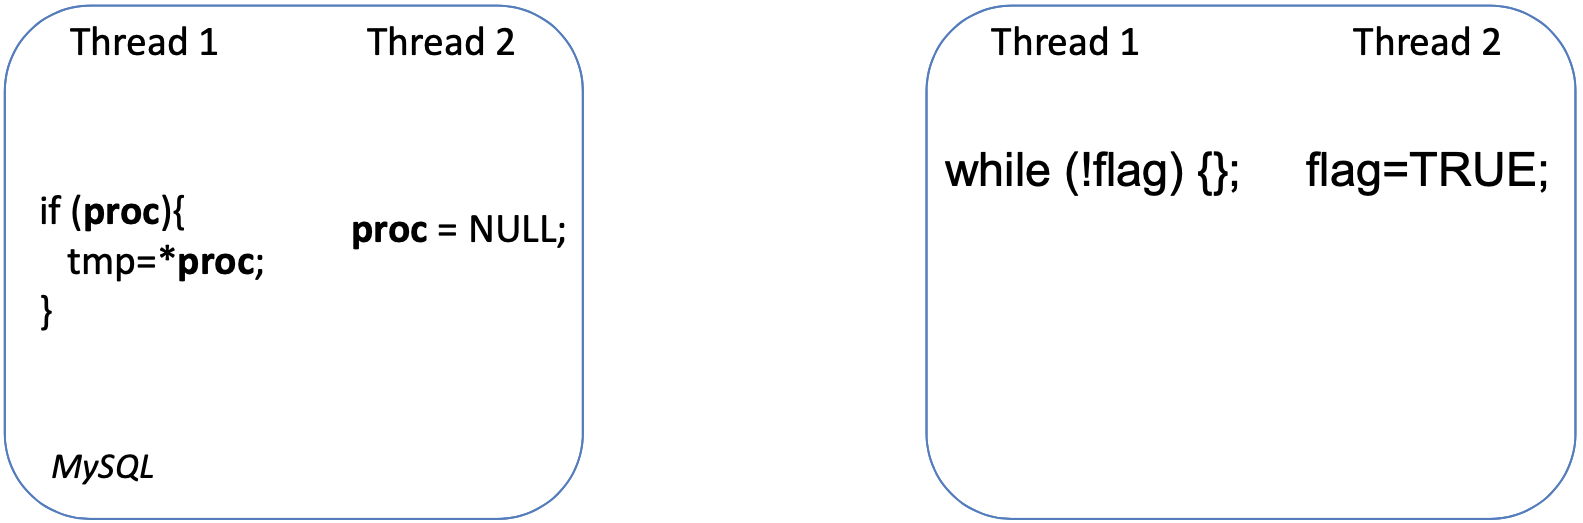
\includegraphics[width=0.6\linewidth]{figs/atomic-region.png}
%    \caption{xxxx}
    \end{figure}
\end{frame}
%----------------------------------------------
% ####  How to detect atomicity‐violations?
% 
% 20200407-lecture2.zip-Lec2.pdf-P43
% 
% Know which code region should maintain atomicity
% 
% ![atomicity](figs/atomicity.png)
% 
% Judge whether a code region’s atomicity is violated
% 
% ![atomic-region](figs/atomic-region.png)
% 
% 
% 
%----------------------------------------------
\begin{frame}
\frametitle{提纲} % Table of contents slide, comment this block out to remove it
\tableofcontents % Throughout your presentation, if you choose to use \section{} and \subsection{} commands, these will automatically be printed on this slide as an overview of your presentation

Ref: Shan Lu, \href{https://s4plus.ustc.edu.cn/_upload/article/files/84/48/964812c049829f4538793b862187/430bcb14-7aa7-4689-b340-9c81e735e5eb.pdf}{Detecting and Fixing Concurrency Bugs}, University of Chicago

\end{frame}
%----------------------------------------------
\subsection{AVIO} % A subsection can be created just before a set of slides with a common theme to further break down your presentation into chunks
%----------------------------------------------
\begin{frame}[fragile]
    \frametitle{AVIO: \small{Detecting Atomicity Violations via Access-Interleaving Invariants (\href{https://sites.cs.ucsb.edu/~arch/spr07-seminar/papers/avio-asplos06.pdf}{ASPLOS’06})}}
%    \framesubtitle{xxxx}

Atomicity violation = unserializable interleaving

%% figure
    \begin{figure}
    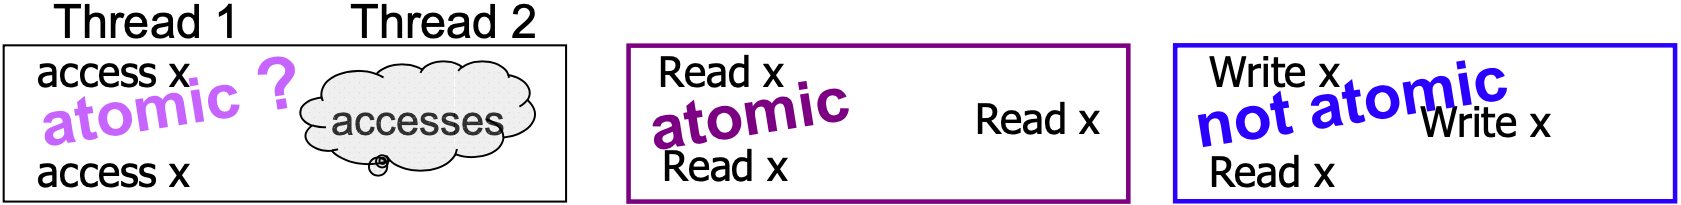
\includegraphics[width=1.0\linewidth]{figs/serialization.png}
%    \caption{xxxx}
    \end{figure}
\end{frame}
%----------------------------------------------
% ### AVIO: Detecting Atomicity Violations via Access-Interleaving Invariants (ASPLOS’06)
% 
% 20200407-lecture2.zip-Lec2.pdf-P45-46
% 
% #### Atomicity violation
% 
% Atomicity violation = unserializable interleaving
% 
% ![serialization](figs/serialization.png)
% 
%----------------------------------------------
\begin{frame}[fragile]
    \frametitle{AVIO: \small{Detecting Atomicity Violations via Access-Interleaving Invariants (ASPLOS’06)}}
%    \framesubtitle{xxxx}

Totally 8 cases of interleaving

%% figure
    \begin{figure}
    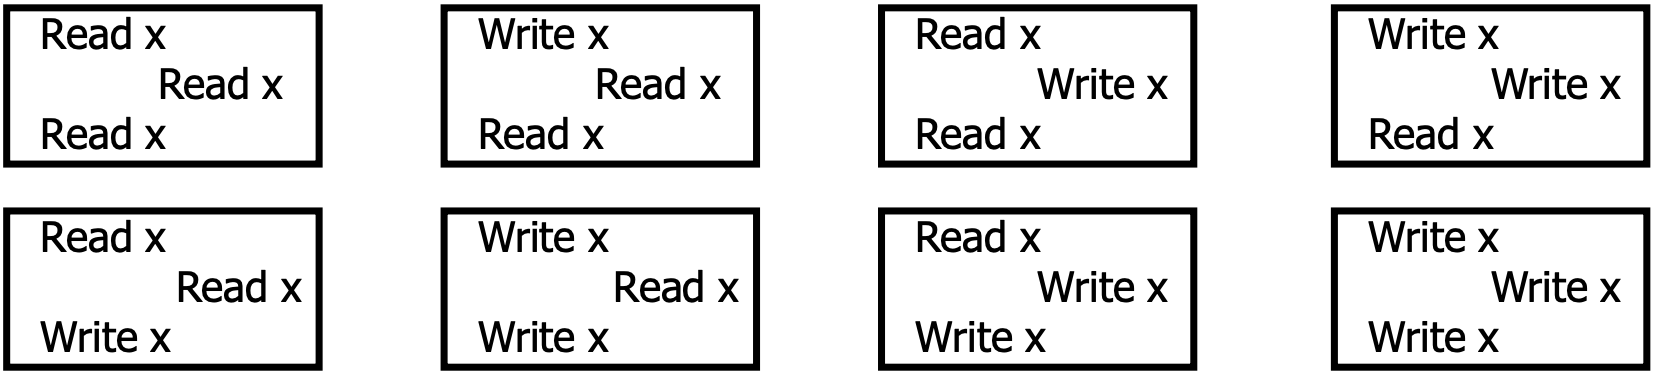
\includegraphics[width=1.0\linewidth]{figs/interleaving-cases.png}
%    \caption{xxxx}
    \end{figure}
\end{frame}
%----------------------------------------------
% #### Read/Write interleaving
% 
% Totally 8 cases of interleaving
% 
% ![interleaving-cases](figs/interleaving-cases.png)
% 
%----------------------------------------------
\begin{frame}[fragile]
    \frametitle{AVIO: \small{Detecting Atomicity Violations via Access-Interleaving Invariants (ASPLOS’06)}}
%    \framesubtitle{xxxx}

4 out of 8 cases are interleaving violations

%% figure
    \begin{figure}
    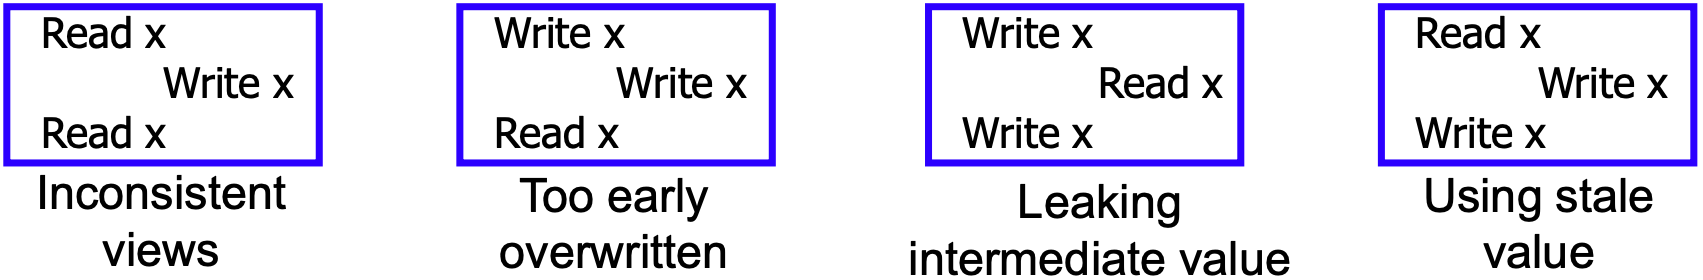
\includegraphics[width=1.0\linewidth]{figs/interleaving-violations.png}
%    \caption{xxxx}
    \end{figure} \pause

Both hardware and software solutions exist

\end{frame}
%----------------------------------------------
% #### Interleaving violations
% 
% 4 out of 8 cases are interleaving violations
% 
% ![interleaving-violations](figs/interleaving-violations.png)
% 
% 
% Both hardware and software solutions exist
% 
% 
% 
%----------------------------------------------
\begin{frame}
\frametitle{提纲} % Table of contents slide, comment this block out to remove it
\tableofcontents % Throughout your presentation, if you choose to use \section{} and \subsection{} commands, these will automatically be printed on this slide as an overview of your presentation

Ref: Shan Lu, \href{https://s4plus.ustc.edu.cn/_upload/article/files/84/48/964812c049829f4538793b862187/430bcb14-7aa7-4689-b340-9c81e735e5eb.pdf}{Detecting and Fixing Concurrency Bugs}, University of Chicago

\end{frame}
%----------------------------------------------
\subsection{ConSeq \& ConMem} % A subsection can be created just before a set of slides with a common theme to further break down your presentation into chunks
%----------------------------------------------
\begin{frame}[fragile]
    \frametitle{ConSeq \& ConMem}
%    \framesubtitle{xxxx}
%% figure
    \begin{figure}
    
\includegraphics[width=0.85\linewidth]{figs/ConSeq-idea.png}
%    \caption{xxxx}
    \end{figure} \pause

    \begin{itemize}
	    \item ConMem
    	\begin{itemize}
    	    \item Detecting Severe Concurrency Bugs through an Effect-Oriented Approach, \href{https://people.cs.uchicago.edu/~shanlu/paper/asplos184-zhang.pdf}{ASPLOS’10}
    	\end{itemize} \pause
	    \item ConSeq
    	\begin{itemize}
    	    \item Detecting Concurrency Bugs through Sequential Errors, \href{https://research.cs.wisc.edu/wpis/papers/asplos11.pdf}{ASPLOS’11}
    	\end{itemize}
	\end{itemize}
\end{frame}
%----------------------------------------------

% ### ConSeq & ConMem
% 
% #### University of Chicago Tools: ConSeq & ConMem
% 20200407-lecture2.zip-Lec2.pdf-P62
% 
% ![ConSeq-idea](figs/ConSeq-idea.png)
% 
% 20200407-lecture2.zip-Lec2.pdf-P71
% 
%----------------------------------------------
\begin{frame}[fragile]
    \frametitle{The lifecycle of concurrency bugs: Fault}
%    \framesubtitle{xxxx}
%% figure
    \begin{figure}
    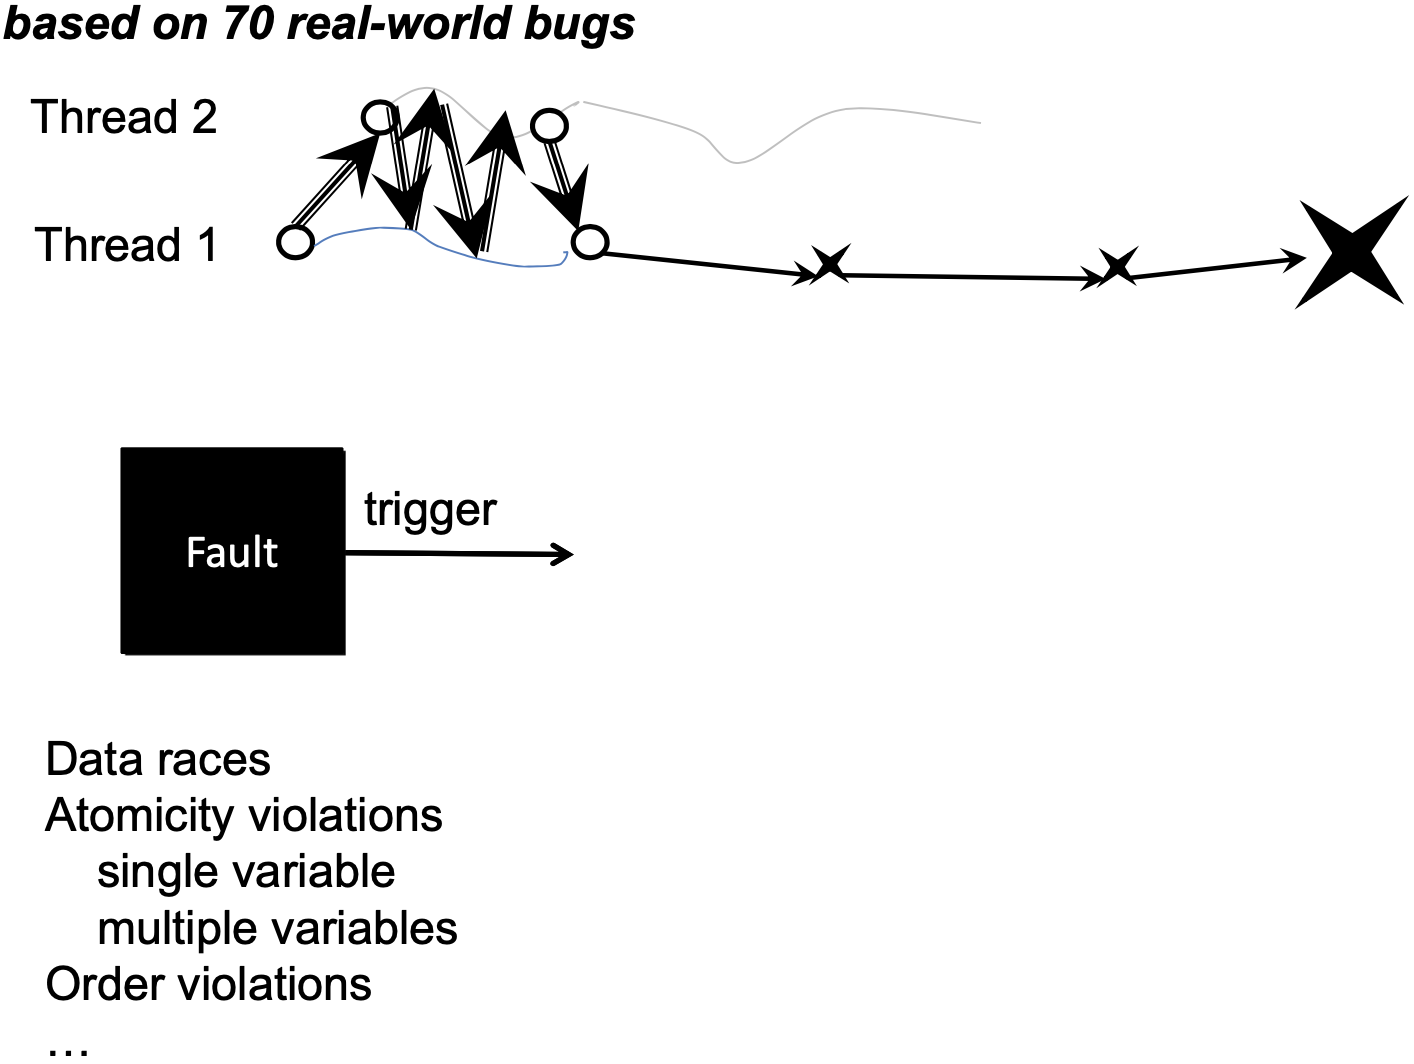
\includegraphics[width=0.62\linewidth]{figs/fault.png}
%    \caption{xxxx}
    \end{figure}
\end{frame}
%----------------------------------------------
% #### The lifecycle of concurrency bugs: Fault
% 20200407-lecture2.zip-Lec2.pdf-P63-66
% 
% ![fault](figs/fault.png)
% 
%----------------------------------------------
\begin{frame}[fragile]
    \frametitle{The lifecycle of concurrency bugs: Error}
%    \framesubtitle{xxxx}
%% figure
    \begin{figure}
    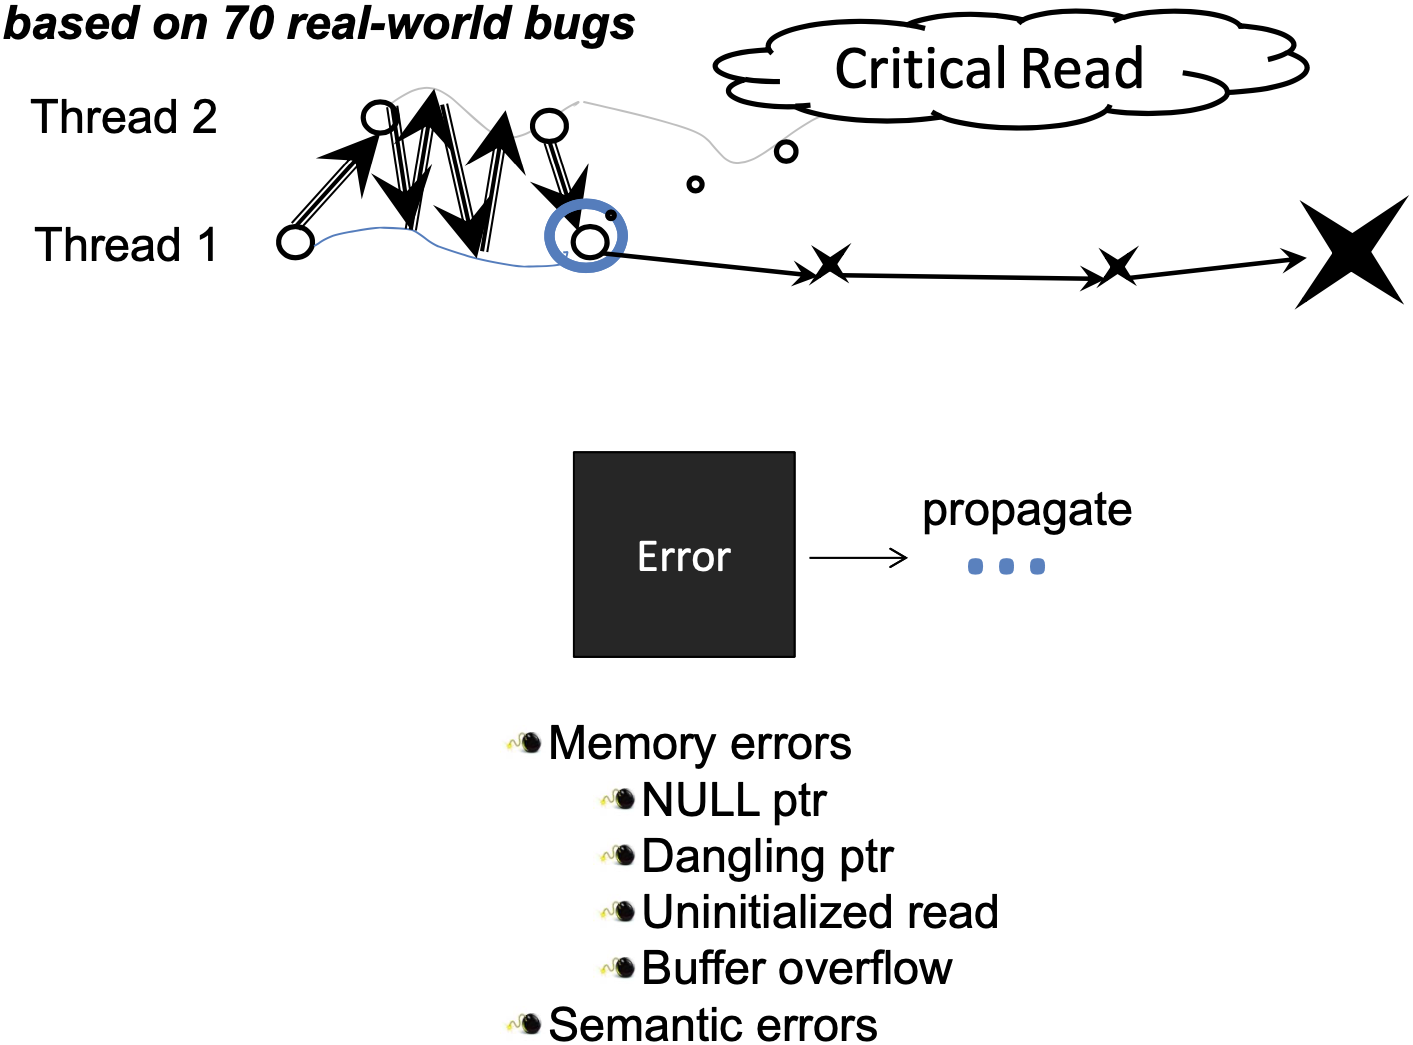
\includegraphics[width=0.6\linewidth]{figs/error.png}
%    \caption{xxxx}
    \end{figure}
\end{frame}
%----------------------------------------------
% #### The lifecycle of concurrency bugs: Error
% 20200407-lecture2.zip-Lec2.pdf-P63-66
% 
% ![error](figs/error.png)
% 
%----------------------------------------------
\begin{frame}[fragile]
    \frametitle{The lifecycle of concurrency bugs: Failure}
%    \framesubtitle{xxxx}
%% figure
    \begin{figure}
    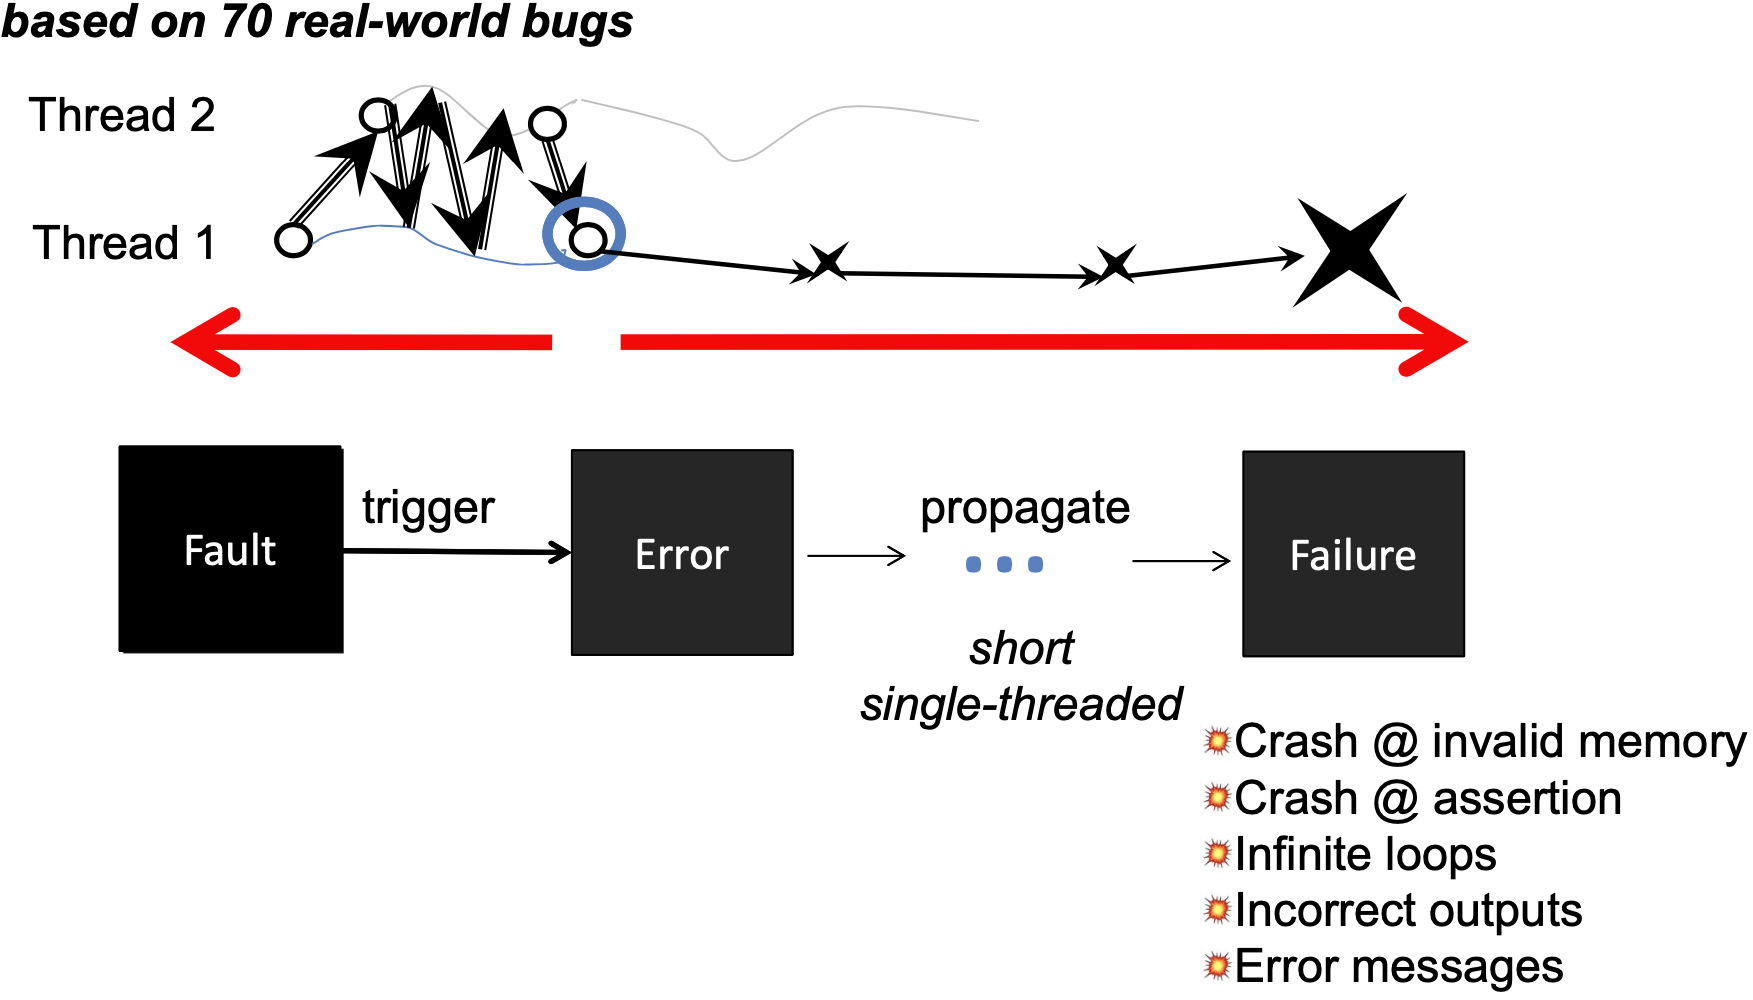
\includegraphics[width=0.75\linewidth]{figs/failure.png}
%    \caption{xxxx}
    \end{figure}
\end{frame}
%----------------------------------------------
% #### The lifecycle of concurrency bugs: Failure
% 20200407-lecture2.zip-Lec2.pdf-P63-66
% 
% ![failure](figs/failure.png)
% 
%----------------------------------------------
\begin{frame}[fragile]
    \frametitle{Cause‐oriented approach}
%    \framesubtitle{xxxx}
%% figure
    \begin{figure}
    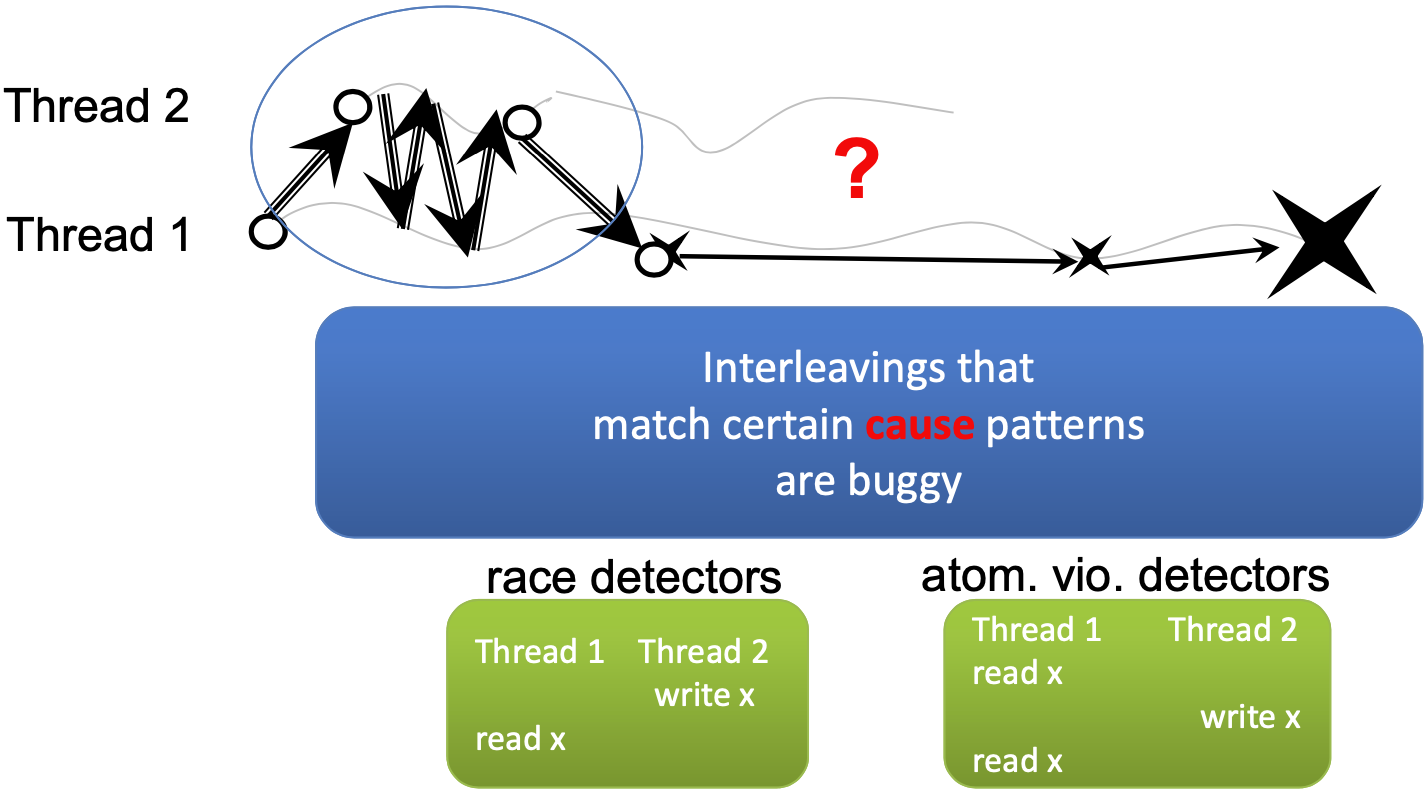
\includegraphics[width=0.55\linewidth]{figs/cause-oriented-approach.png}
%    \caption{xxxx}
    \end{figure} \pause
	\begin{block}{Limitations}

        \begin{itemize}
            \item False positives
            \item False negatives
        \end{itemize}
    \end{block}
\end{frame}
%----------------------------------------------
% #### Cause‐oriented approach
% 20200407-lecture2.zip-Lec2.pdf-P69
% Limitations
% – False positives
% – False negatives
% 
% ![cause-oriented-approach](figs/cause-oriented-approach.png)
% 
% 
% 
%----------------------------------------------
\begin{frame}[fragile]
    \frametitle{Effect‐oriented approach}
%    \framesubtitle{xxxx}
%% figure
    \begin{figure}
    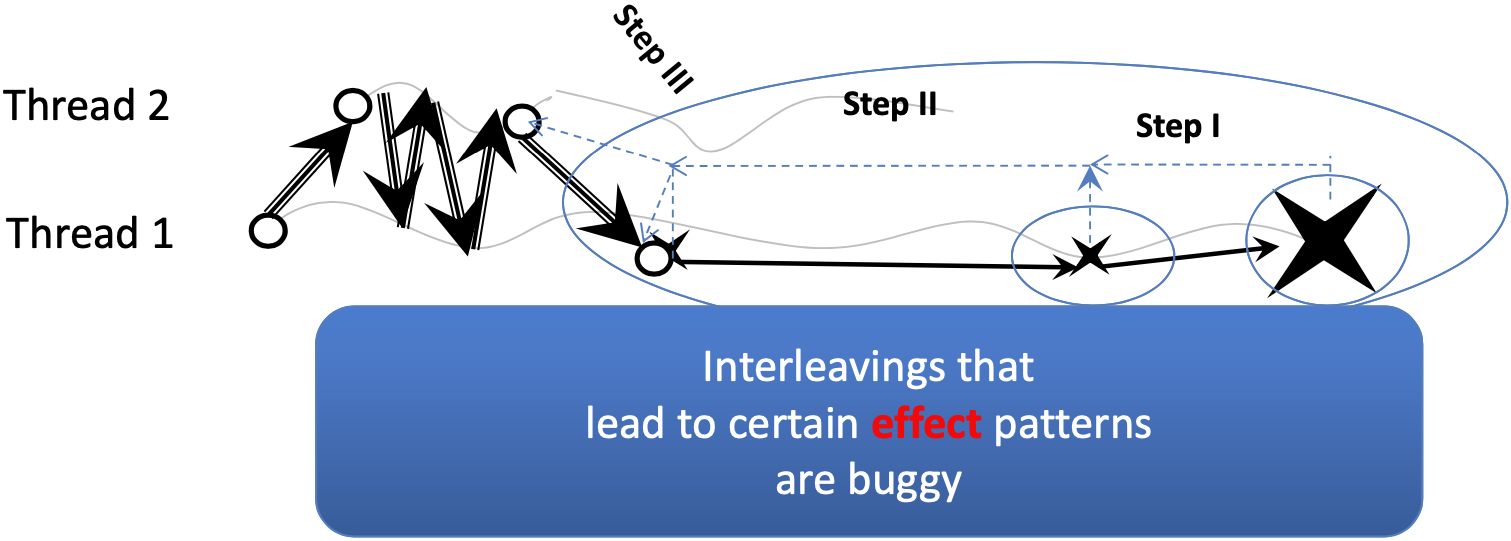
\includegraphics[width=0.7\linewidth]{figs/Effect‐oriented-approach.png}
%    \caption{xxxx}
    \end{figure} \pause

    \begin{itemize}
        \item Step 1: Statically identify potential failure/error site \pause
        \item Step 2: Statically look for critical reads \pause
        \item Step 3: Dynamically identify buggy interleaving
    \end{itemize}

\end{frame}
%----------------------------------------------
% #### Effect‐oriented approach
% 
% 20200407-lecture2.zip-Lec2.pdf-P70
% 
% – Step 1: *Statically* identify potential failure/error site
% 
% – Step 2: *Statically* look for critical reads
% – Step 3: *Dynamically* identify buggy interleaving
% 
% ![Effect‐oriented-approach](figs/Effect‐oriented-approach.png)
% 
%----------------------------------------------
\begin{frame}[fragile]
    \frametitle{ConMem}
    \framesubtitle{Detecting Severe Concurrency Bugs through an Effect-Oriented Approach, ASPLOS’10}
%% figure
    \begin{figure}
    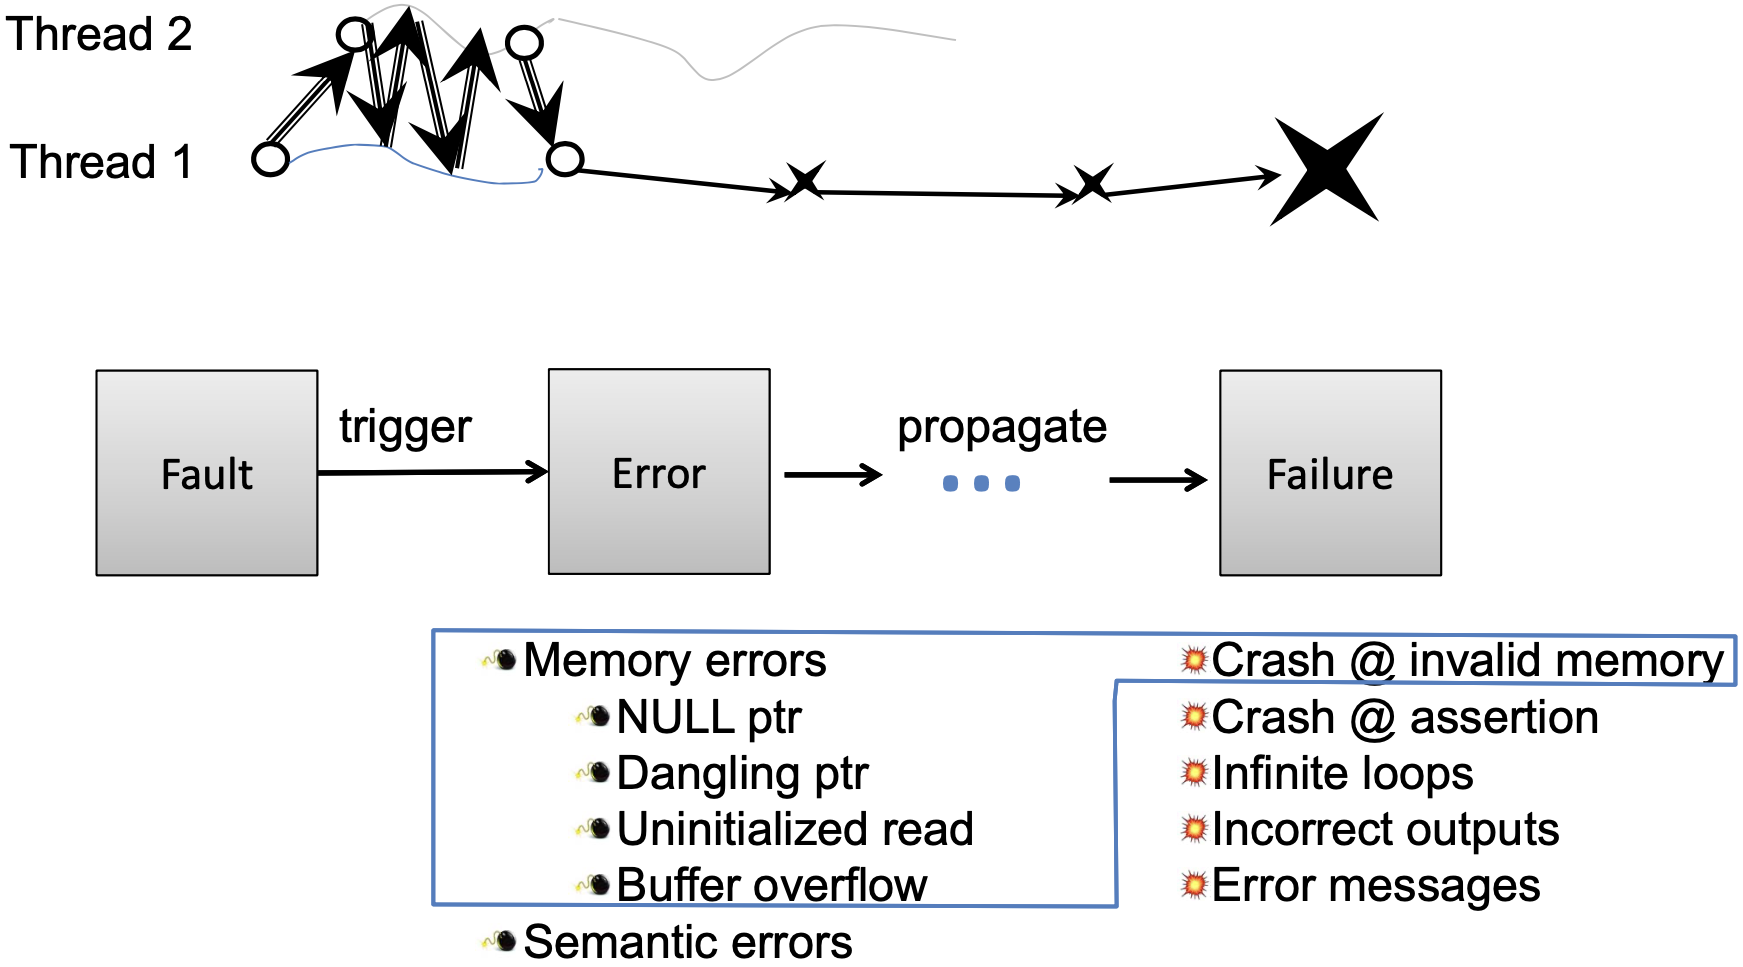
\includegraphics[width=0.73\linewidth]{figs/ConMem.png}
%    \caption{xxxx}
    \end{figure}
\end{frame}
%----------------------------------------------
% #### ConMem: Detecting Severe Concurrency Bugs through an Effect-Oriented Approach, ASPLOS’10
% 20200407-lecture2.zip-Lec2.pdf-P72
% 
% ![ConMem](figs/ConMem.png)
% 
% 
%----------------------------------------------
\begin{frame}[fragile]
    \frametitle{ConSeq: \small{Detecting Concurrency Bugs through Sequential Errors, ASPLOS’11}}
%    \framesubtitle{xxxx}
%% figure
    \begin{figure}
    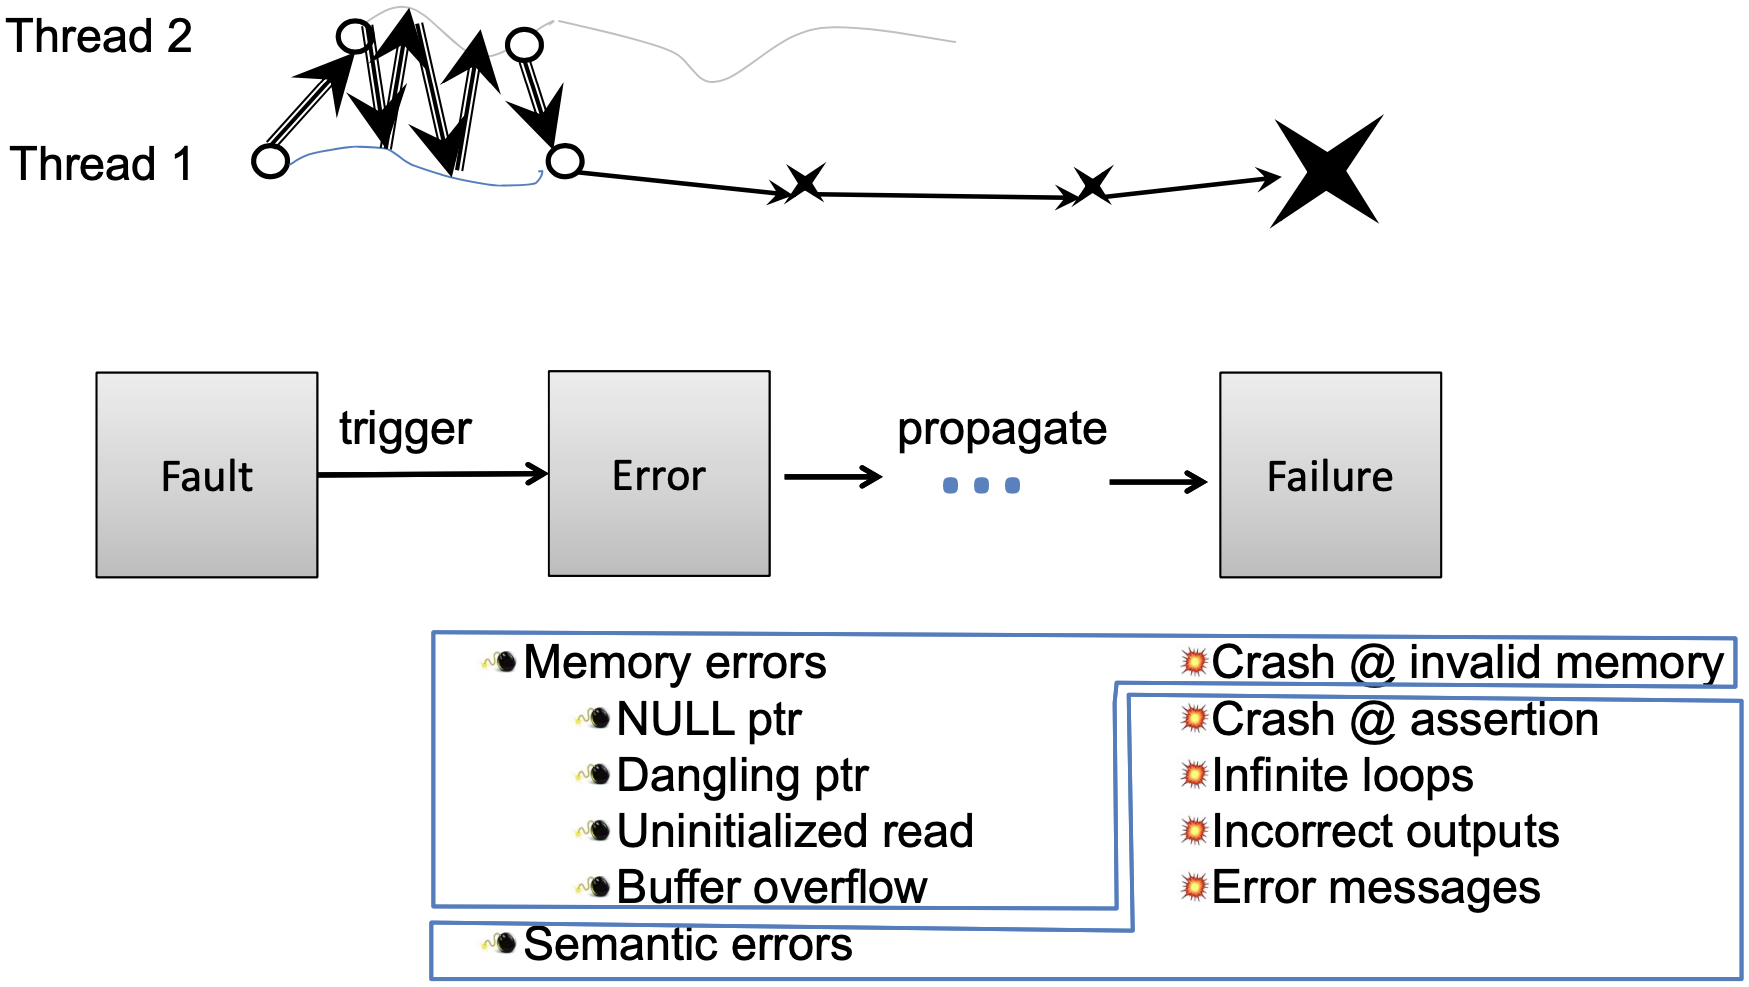
\includegraphics[width=0.75\linewidth]{figs/ConSeq.png}
%    \caption{xxxx}
    \end{figure}
\end{frame}
%----------------------------------------------
% #### ConSeq: Detecting Concurrency Bugs through Sequential Errors, ASPLOS’11
% 20200407-lecture2.zip-Lec2.pdf-P73
% 
% ![ConSeq](figs/ConSeq.png)
%----------------------------------------------
\end{document}
